%!TEX root = ../thesis.tex
%*******************************************************************************
%*********************************** First Chapter *****************************
%*******************************************************************************

\chapter{Introduction}  %Title of the First Chapter

\ifpdf
    \graphicspath{{Chapter1/Figs/Raster/}{Chapter1/Figs/PDF/}{Chapter1/Figs/}}
\else
    \graphicspath{{Chapter1/Figs/Vector/}{Chapter1/Figs/}}
\fi


%********************************** %First Section  **************************************
\section{Credit Card Fraud} %Section - 1.1 

\subsection{Definition and impact of Credit Card Fraud}

A Criminal Code \citep{criminal380} which is a law that codifies most criminal offenses and procedures in Canada, section 380 provides the general definition for fraud in Canada:

\begin{enumerate}
\item Every one who, by deceit, falsehood or other fraudulent means, whether or not it is a false pretense within the meaning of this Act, defrauds the public or any person, whether ascertained or not, of any property, money or valuable security or any service,

\begin{enumerate}
\item is guilty of an indictable offense and liable to a term of imprisonment not exceeding fourteen years, where the subject-matter of the offense is a testamentary instrument or the value of the subject-matter of the offense exceeds five thousand dollars; or
\item is guilty

\begin{enumerate}
\item of an indictable offense and is liable to imprisonment for a term not exceeding two years, or
\item of an offense punishable on summary conviction, where the value of the subject-matter of the offense does not exceed five thousand dollars.
\end{enumerate}

\end{enumerate}

\end{enumerate}


In recent years, e-commerce has gained a lot in popularity mainly due to the ease of cross-border purchases and online credit card transactions. While e-commerce is already a mature business with many players, security for online payment lags behind. With an extensive use of credit cards, fraud seems like a major issue in the credit card business. It is not easy to see the impact of fraud since companies and banks have a good motivation not to disclose a full report of losses due to frauds. However, as stated in the Lexis Nexis's study \citep{lexisnexis2014}, in 2014 fraudulent card transactions worldwide have reached around \$11 billion a year. A latest study of Lexis Nexis \citep{lexisnexis2016} estimated that a cost of fraud as a percentage of revenues keeps going up, from 0.51\% in 2013 increasing to 1.47\% in 2016 (Figure \ref{cost_of_fraud_as_percentage_revenues}), and a total costs of fraud losses for each dollar is up to 2.4 times (Figure \ref{total_cost_per_dollar}). In the United Kingdom, total losses through credit card fraud have been growing rapidly from £122 million in 1997 to £440.3 million in 2010 according to an estimation of the Association for Payment Clearing Services (APACS) \cite{delamaire2009credit}.


\begin{figure}
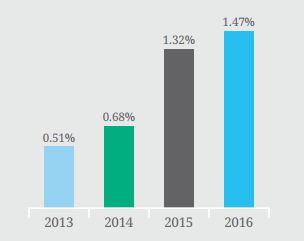
\includegraphics[scale=0.8]{Images/cost_of_fraud_as_percentage_of_revenues.png}
\centering
\caption{Cost of Fraud as a \% of Revenues Keeps Going Up \citep{lexisnexis2016}}
\label{cost_of_fraud_as_percentage_revenues}
\end{figure}



\begin{figure}
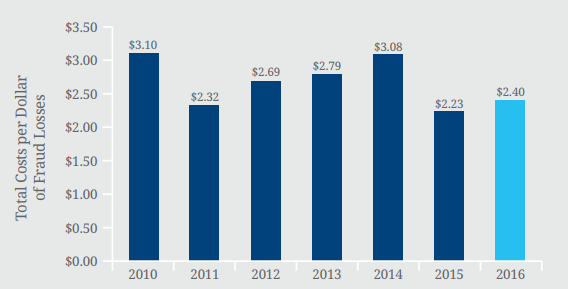
\includegraphics[width=\textwidth]{Images/total_costs_per_dollar_of_fraud.png}
\centering
\caption{Total Costs per Dollar of Fraud Losses \citep{lexisnexis2016}}
\label{total_cost_per_dollar}
\end{figure}


There are many types of fraud, but in this thesis we focus on credit card fraud. The credit card frauds might occur in several ways, for instance:

\begin{itemize}
\item Card-holder-not-present fraud is a payment card transaction made where the card-holder doesn't or can't physically present the card for a merchant's visual examination at the time that an order is given and payment effected, for example a transaction is ordered via mail, telephone or Internet,
\item Stolen card fraud is the most common type of fraud where the stolen card may be used for illegal purchases as much as possible and as quickly as possible until the card holder notifies and blocks the account.
\end{itemize}


\subsection{Credit Card Fraud Detection}

Detecting credit card fraud attracts a lot of attention from industry (bank, insurance, \dots) and from the research community for the last three decades. The fraud detection process is based on the analysis of recorded transactions, which are a set of attributes (for example identifier, transaction timestamp, amount of the transaction, \dots). Traditional methods of data analysis have long been used to detect fraud, it requires large human resource, time-consuming inquiry, wide range of knowledge to analyze a huge number of transactions. However, the human resource is limited and thus automatic fraud detection system is really necessary because it is not easy for a human analyst to detect fraudulent patterns in transaction datasets with a huge number of samples and many attributes. With a rising of Machine Learning field, which is able to learn patterns from data automatically and have been applied in several applications, this is a suitable approach for fraud detection problem. However, a design for the Fraud Detection System (FDS) is particularly challenging for several reasons:

\begin{itemize}
\item The number of credit card frauds is really small - a tiny fraction of all the daily transactions. Many algorithms in Machine Learning have not been designed to deal with this problem,
\item Many fraud transactions have an insignificant difference to normal transactions, which makes these transactions hard to detect by Machine Learning algorithms,
\item Over the time, new attack strategies are created and changes in customer behavior make the distribution of data change over time and it does not meet the basic assumption in Machine Learning (as well as Statistics),
\item \dots.
\end{itemize}


\section{Contributions}

Focusing on the credit card fraud detection problem and some other related issues, in this thesis we present a series of independent contributions through this thesis, including:


\subsection*{Fraud Detection Pipeline}

Despite rich literature on fraud detection, there is no agreement on what is the best way to solve this problem and also there is no public fraud detection system. This means that in the industry, when a company wants to build their own a fraud detection system, they cannot decide which is a good way to do so, especially for those companies in Vietnam. The first main contribution of this thesis is a survey on the fraud detection problem, we will show readers several challenges in building the Fraud Detection System. Based on that, we propose one system that not only good but also simple that companies could implement by themselves easily, which we call Fraud Detection Pipeline. Furthermore, we give readers many possible ways to extend the system.


\subsection*{Update Point Estimation for the case of Concept-Drift in fraud detection problem}

Fraudsters always try to create new fraud strategies and normal customers usually change their behavior, these changes make non-fraud/fraud patterns in our dataset change over time. In this case, the system has to update its models frequently to keep its accuracy, either on a daily or a less frequent period. With the credit card fraud detection problem, a common choice is daily when we receive a daily full dataset and then update the models at night. However, updating models daily is worthless and actually it is only necessary when we do not have to adapt to new fraudulent patterns. In other words, we should update models if and only if it makes an improvement to our system. The second contribution is a mechanism that helps us make a decision on when we should update our models.


\subsection*{K-Segments Under Bagging approach: An experimental Study on Extremely Imbalanced Data Classification}

Imbalanced dataset could be found in many real-world domains, e.g. fraud detection problem, and there are several methods have been proposed to handle the imbalance problem, but there is no guarantee those methods will work with an extreme imbalance case. Big Data is a problem concerning the volume and the complexity of data, whereas the big data in extremely imbalance data is a different problem from those original issues that attracts much attention recently. In this study, as the third contribution, we show that a simplified combination of under-sampling and ensemble learning is very effective in the case mentioned.


\subsection*{Solve fraud detection problem by using graph based learning methods}

To detect the credit cards' fraud transactions, data scientists normally employ the un-supervised learning techniques and supervised learning technique. Among several algorithms that have been proposed for this problem, a graph-based semi-supervised learning have not been applied to the credit cards' fraudulent transactions detection before. We propose to apply an un-normalized graph p-Laplacian based semi-supervised learning technique combined with an undersampling technique to find a relationship of those frauds in the data.


\section{Outline}

This thesis is organized as follows:

\begin{itemize}
\item Chapter 2 prepares the necessary knowledge which would be helpful for the next chapters,
\item Chapter 3 reviews several challenges of the fraud detection problem and their possible solutions, based on that we select the most suitable approaches and combine them into one best strategy as in our proposed Fraud Detection Pipeline,
\item Chapter 4 uses the Fraud Detection Pipeline and presents a mechanism to detects which model need to update to keep the accuracy of our system and also reduces the update cost,
\item Chapter 5 explains more details of our selected techniques in the pipeline how they are useful to us in the case of the extremely imbalanced big dataset,
\item And finally, chapter 7 summarizes our results and proposes future research directions.
\end{itemize}
